%%%%%%%%%%%%%%%%%%%%%%%%%%%%%%%%%%%%%%%%%
% Structured General Purpose Assignment
% LaTeX Template
%
% This template has been downloaded from:
% http://www.latextemplates.com
%
% Original author:
% Ted Pavlic (http://www.tedpavlic.com)
%
% Note:
% The \lipsum[#] commands throughout this template generate dummy text
% to fill the template out. These commands should all be removed when 
% writing assignment content.
%
%%%%%%%%%%%%%%%%%%%%%%%%%%%%%%%%%%%%%%%%%

%----------------------------------------------------------------------------------------
%	PACKAGES AND OTHER DOCUMENT CONFIGURATIONS
%----------------------------------------------------------------------------------------

\documentclass{article}

\usepackage{fancyhdr} % Required for custom headers
\usepackage{lastpage} % Required to determine the last page for the footer
\usepackage{extramarks} % Required for headers and footers
\usepackage{graphicx} % Required to insert images
\usepackage{lipsum} % Used for inserting dummy 'Lorem ipsum' text into the template
\usepackage{algorithm, algpseudocode}

\usepackage{bera}% optional: just to have a nice mono-spaced font
\usepackage{listings}
\usepackage{xcolor}

\colorlet{punct}{red!60!black}
\definecolor{background}{HTML}{EEEEEE}
\definecolor{delim}{RGB}{20,105,176}
\colorlet{numb}{magenta!60!black}

\lstdefinelanguage{json}{
	basicstyle=\normalfont\ttfamily,
	numbers=left,
	numberstyle=\scriptsize,
	stepnumber=1,
	numbersep=8pt,
	showstringspaces=false,
	breaklines=true,
	frame=lines,
	backgroundcolor=\color{background},
	literate=
	*{0}{{{\color{numb}0}}}{1}
	{1}{{{\color{numb}1}}}{1}
	{2}{{{\color{numb}2}}}{1}
	{3}{{{\color{numb}3}}}{1}
	{4}{{{\color{numb}4}}}{1}
	{5}{{{\color{numb}5}}}{1}
	{6}{{{\color{numb}6}}}{1}
	{7}{{{\color{numb}7}}}{1}
	{8}{{{\color{numb}8}}}{1}
	{9}{{{\color{numb}9}}}{1}
	{:}{{{\color{punct}{:}}}}{1}
	{,}{{{\color{punct}{,}}}}{1}
	{\{}{{{\color{delim}{\{}}}}{1}
	{\}}{{{\color{delim}{\}}}}}{1}
	{[}{{{\color{delim}{[}}}}{1}
	{]}{{{\color{delim}{]}}}}{1},
}

% Margins
\topmargin=-0.45in
\evensidemargin=0in
\oddsidemargin=0in
\textwidth=6.5in
\textheight=9.0in
\headsep=0.25in 

\linespread{1.1} % Line spacing

% Set up the header and footer
\pagestyle{fancy}
\lhead{\hmwkAuthorName} % Top left header
\chead{\hmwkClass\ (\hmwkClassInstructor\ \hmwkClassTime): \hmwkTitle} % Top center header
\rhead{\firstxmark} % Top right header
\lfoot{\lastxmark} % Bottom left footer
\cfoot{} % Bottom center footer
\rfoot{Page\ \thepage\ of\ \pageref{LastPage}} % Bottom right footer
\renewcommand\headrulewidth{0.4pt} % Size of the header rule
\renewcommand\footrulewidth{0.4pt} % Size of the footer rule

\setlength\parindent{0pt} % Removes all indentation from paragraphs

%----------------------------------------------------------------------------------------
%	DOCUMENT STRUCTURE COMMANDS
%	Skip this unless you know what you're doing
%----------------------------------------------------------------------------------------

% Header and footer for when a page split occurs within a problem environment
\newcommand{\enterProblemHeader}[1]{
\nobreak\extramarks{#1}{#1 continued on next page\ldots}\nobreak
\nobreak\extramarks{#1 (continued)}{#1 continued on next page\ldots}\nobreak
}

% Header and footer for when a page split occurs between problem environments
\newcommand{\exitProblemHeader}[1]{
\nobreak\extramarks{#1 (continued)}{#1 continued on next page\ldots}\nobreak
\nobreak\extramarks{#1}{}\nobreak
}

\setcounter{secnumdepth}{0} % Removes default section numbers
\newcounter{homeworkProblemCounter} % Creates a counter to keep track of the number of problems

\newcommand{\homeworkProblemName}{}
\newenvironment{homeworkProblem}[1][Problem \arabic{homeworkProblemCounter}]{ % Makes a new environment called homeworkProblem which takes 1 argument (custom name) but the default is "Problem #"
\stepcounter{homeworkProblemCounter} % Increase counter for number of problems
\renewcommand{\homeworkProblemName}{#1} % Assign \homeworkProblemName the name of the problem
\section{\homeworkProblemName} % Make a section in the document with the custom problem count
\enterProblemHeader{\homeworkProblemName} % Header and footer within the environment
}{
\exitProblemHeader{\homeworkProblemName} % Header and footer after the environment
}

\newcommand{\problemAnswer}[1]{ % Defines the problem answer command with the content as the only argument
\noindent\framebox[\columnwidth][c]{\begin{minipage}{0.98\columnwidth}#1\end{minipage}} % Makes the box around the problem answer and puts the content inside
}

\newcommand{\homeworkSectionName}{}
\newenvironment{homeworkSection}[1]{ % New environment for sections within homework problems, takes 1 argument - the name of the section
\renewcommand{\homeworkSectionName}{#1} % Assign \homeworkSectionName to the name of the section from the environment argument
\subsection{\homeworkSectionName} % Make a subsection with the custom name of the subsection
\enterProblemHeader{\homeworkProblemName\ [\homeworkSectionName]} % Header and footer within the environment
}{
\enterProblemHeader{\homeworkProblemName} % Header and footer after the environment
}
   
%----------------------------------------------------------------------------------------
%	NAME AND CLASS SECTION
%----------------------------------------------------------------------------------------

\newcommand{\hmwkTitle}{Project\ \#1} % Assignment title
\newcommand{\hmwkDueDate}{Friday,\ August\ 7,\ 2015} % Due date
\newcommand{\hmwkClass}{NWEN\ 406} % Course/class
%\newcommand{\hmwkClassTime}{10:30am} % Class/lecture time
%\newcommand{\hmwkClassInstructor}{Jones} % Teacher/lecturer
\newcommand{\hmwkAuthorName}{Boxiong Tan} % Your name

%----------------------------------------------------------------------------------------
%	TITLE PAGE
%----------------------------------------------------------------------------------------

\title{
\vspace{2in}
\textmd{\textbf{\hmwkClass:\ \hmwkTitle}}\\
\normalsize\vspace{0.1in}\small{Due\ on\ \hmwkDueDate}\\
\vspace{0.1in}\large{\textit{\hmwkClassInstructor\ \hmwkClassTime}}
\vspace{3in}
}

\author{\textbf{\hmwkAuthorName}}
\date{} % Insert date here if you want it to appear below your name

%----------------------------------------------------------------------------------------

\begin{document}

\maketitle

%----------------------------------------------------------------------------------------
%	TABLE OF CONTENTS
%----------------------------------------------------------------------------------------

%\setcounter{tocdepth}{1} % Uncomment this line if you don't want subsections listed in the ToC

%\newpage
%\tableofcontents
%\newpage

%----------------------------------------------------------------------------------------
%	PROBLEM 1
%----------------------------------------------------------------------------------------

% To have just one problem per page, simply put a \clearpage after each problem

\begin{homeworkProblem}[Project Objectives]
\begin{enumerate}
	\item Obtain an Amazon AWS micro-instance and configure it.
	\item Write a server which could receive and send messages.
\end{enumerate}
%\lipsum[1]\vspace{10pt} % Question
\end{homeworkProblem}

\begin{homeworkProblem}[Micro-instance Configuration]
\problemAnswer{ % Answer
%\begin{center}
%
\includegraphics[width=0.75\columnwidth]{example_figure} % Example image
%\end{center}
Major steps of configuration:

\begin{enumerate}
	\item Choose an Amazon Machine Image (AMI) $\rightarrow$ \textbf{Ubuntu Server}
	\item Choose an instance Type $\rightarrow$ \textbf{t2.micro}
	\item Configure instance Details

		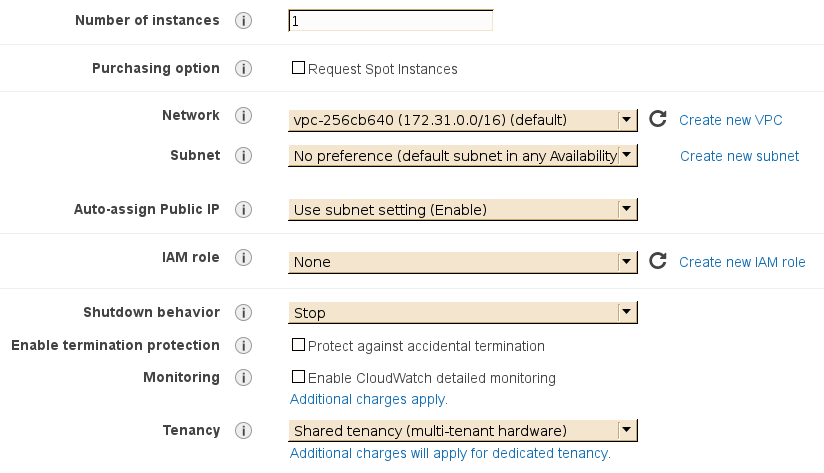
\includegraphics[width=0.75\columnwidth]{pics/step3.png}
	\item Add storage $\rightarrow$ \textbf{8 GB General Purpose (SSD)}
	\item Tag Instance $\rightarrow$ \textbf{``Max'':``MyServer''}
	\item Configure Security Group $\rightarrow$ \textbf{All traffic}
\end{enumerate}

After configuration, launch the micro-instance.
\begin{center}
	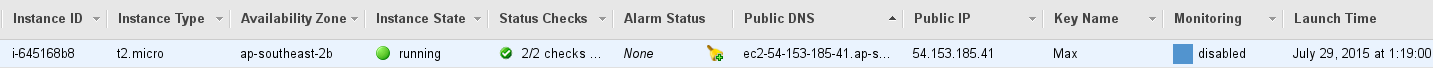
\includegraphics[width=1\columnwidth]{pics/micro-instance.png}
\end{center}

%\lipsum[2]
}
\end{homeworkProblem}

%----------------------------------------------------------------------------------------
%	PROBLEM 2
%----------------------------------------------------------------------------------------

\begin{homeworkProblem}[Web Server] % Custom section title
%\lipsum[3] % Question

%--------------------------------------------

\begin{homeworkSection}{Programming Environment} % Section within problem

Programming language: \textbf{Python v2.7}

Web Server framework: \textbf{Flask v0.10.1}

%\lipsum[4]\vspace{10pt} % Question
%
%\problemAnswer{ % Answer
%\lipsum[5]
%}
\end{homeworkSection}

%--------------------------------------------

\begin{homeworkSection}{Description} % Section within problem

The Restful Web server runs in the background and listening port 80. When receiving a POST request,
it first replies the request by code 202. Then it starts a thread to handle the message. 

For the sake of simplicity, our team decides to pass a json message between members.
This message mainly contains a string message, which each member must edited it when received the message.
Each member could handle this string message with a simple hashing or string mashing algorithm.
	
\begin{algorithm}
	\caption{Web server}
	\begin{algorithmic}
		\State Listen to HTTP request on myIP:80/api
		\If { get POST request}
			\State Start a thread handle the received data
			\State reply the request with ``code 202''
		\EndIf

		\State Thread unpack the received data
		\State Thread identify the input message and reverse the message string
		\State Thread edit the index number and count
		\State Thread Pack the edited message as a dictionary
		\State Thread add edited message dictionary to ``max'' message list 
		\Repeat
			\State Thread pop up the first address in the order listed
			\For { three times} 
				\State and try to send the json package to the address. The request timeout is set to 2 seconds.
			\EndFor
		\Until { Send successfully or order list is empty}
	\end{algorithmic}
\end{algorithm}



\hfill

This is an example of starting message:
\begin{lstlisting}[language=json,firstnumber=1]
{
    "value": "thebeginningvalue",
    "count": 0,
    "audit": {},
    "order": [
        "52.25.73.1",
        "52.25.246.56",
        "52.25.246.34",
        "52.25.185.43",
        "52.25.56.34",
        "52.25.127.88"
    ]
}
\end{lstlisting}

The string message allows characters for input and output are 0-9a-zA-Z. 
The output at least one character and maximum of 255. i.e. /[0-9a-zA-Z]{1,255}$/

The order of message passing is completely decide by the ``order'' list predefined by the first sender.
If one of the node in the list failed to response, it will be discarded after three times of trying.

\end{homeworkSection}

%--------------------------------------------

\begin{homeworkSection}{Experimental Results} % Section within problem

Sending JSON to next address: 52.27.64.194
\begin{lstlisting}[language=json,firstnumber=1]
{
    "audit": {
        "Alex": [
            {
                "index": 1,
                "input": "blasomething",
                "output": "Areyouoneofthoseboyswhopreferscarstowomen",
                "time": "2015-08-05 22:17:45 GMT + 0"
            }
        ],
        "max": [
            {
                "index": 0,
                "input": "",
                "output": "blasomething",
                "time": "Wed, 05, Aug 2015 22:17:54 GMT"
            }
        ]
    },
    "count": 2,
    "order": [
        "52.27.228.163",
        "54.68.184.120"
    ],
    "value": "Areyouoneofthoseboyswhopreferscarstowomen"
}

\end{lstlisting}
This example shows, ``max'' starts sending the message to ``Alex''. ``Alex'' further forward this message to
52.27.64.194.


\end{hostworkSection}

\end{homeworkProblem}

%----------------------------------------------------------------------------------------
%	PROBLEM 3
%----------------------------------------------------------------------------------------

%\begin{homeworkProblem}[Prob. \Roman{homeworkProblemCounter}] % Roman numerals

%--------------------------------------------

%\begin{homeworkSection}{\homeworkProblemName:~(a)} % Using the problem name elsewhere
%\problemAnswer{ % Answer
%\lipsum[7]
%}
%\end{homeworkSection}

%--------------------------------------------

%\begin{homeworkSection}{\homeworkProblemName:~(b)}
%\lipsum[8]\vspace{10pt} % Question
%
%\problemAnswer{ % Answer
%\lipsum[9]
%}
%\end{homeworkSection}

%--------------------------------------------

%\end{homeworkProblem}

%----------------------------------------------------------------------------------------
%	PROBLEM 4
%----------------------------------------------------------------------------------------

%\begin{homeworkProblem}[Prob. \Roman{homeworkProblemCounter}] % Roman numerals
%\problemAnswer{ % Answer
%\lipsum[10]
%}
%\end{homeworkProblem}

%----------------------------------------------------------------------------------------

\end{document}
